\chapter{Physical Layer Neural Network Framework for Training Data Formation}
\label{chapter3}

We present a novel open-source dataset modification framework designed to study the effect of wireless channels on the training and testing of modulation classifiers employing Neural Networks (NN). Communication systems optimize for capacity by packing information bits very closely together. Consequently, RF datasets contain less redundancy and context than other NN domains such as image and speech classification. As a result, NN performance is poor when brought to implementation if training is not done with datasets properly describing gathered test sets. Our framework pushes datasets through a sequential, parallelized, modular, block-style set of wireless channels, where blocks can be written by operators or pulled from a core library. Utilizing our datasets, we perform analysis of a NN. We determine the NN requires datasets collected by a receiver capable of phase correction to below 4 degrees offset, and Carrier Frequency Offset (CFO) correction to below $\bf{1\%}$ normalized to sample rate to maintain near-peak modulation classification accuracy.

\subsection{Introduction}
\label{sec1}

There exist numerous approaches published in open literature to model wireless channels~\cite{tsb88tia}. Receive chains apply an equally numerous variation of corrections to signals to remove or limit channel effects on data through frame synchronization, CFO correction, timing corrections, and other methods~\cite{rappaport1996wireless}. Contributions to the field are met with scrutiny due to the maturity of these models and correction systems. However, NNs can adjust for nonlinearities unaccounted for by classical communication and information theory\cite{schenk2008rf}. Significant gains can be achieved by breaking the traditionally sequential nature of activities performed by transmit and receive chains~\cite{wymeersch2007iterative}. Additionally, recent NN publications have shown high-capacity learning algorithms that have demonstrated high energy efficiency and computational throughput~\cite{raina2009large}. Consequentially, interest has been expressed~\cite{8054694, wang2017deep} for the use of NNs in physical layer communications. NN applications in the physical layer can be classified into two categories: end-to-end autoencoders that determine unknown hidden layers to recreate an input data layer at an output data layer, and NNs that determine specific design choices of the physical layer.

For any physical layer NN, an often used framework for dataset generation is GNU Radio Companion's (GRC) channel model blocks. Each channel block offers a modular, sequential, parallelized method of dataset manipulation. While a powerful tool, GRCs gpl3 license makes privacy of work difficult for companies with export control and Non-Disclosure Agreements (NDA). Most all blocks must be written by the user which require documentation, upkeep, and time. Additionally, GRC is better at some use cases than others, requiring creativity to generate some datasets. Most importantly, GRC cannot easily and properly construct massive arrays of varied wireless channels.

In~\cite{o2016radio}, a dataset is generated for use in a NN modulation classifier, and interest is expressed for "iteratively better, more complex, and more challenging datasets", which "will be required to help compare, measure, and evaluate these (communication) tasks". It is the fundamental assumption made in supervised learning of a NN that the training data is representative of practical data. That assumption cannot be broken in data partitioning or through a lack of resolution in the distribution of training data. For many NNs, that assumption is broken by the highly unique nature of wireless transmissions, which are varied by a virtually endless number of channel effects.

In this paper, we propose a framework that creates datasets satisfying this assumption through their size and diversity in a computationally efficient, parallelized method. Channel effects are sequentially applied to complex valued datasets in a modular way, where channel blocks are chosen by a configuration file from a library or user created blocks. Channels described by design parameters can be iterated through, achieving thorough file multiplication labeled in a clear and concise way.

This paper presents our framework in section~\ref{sec2}, and discusses implementation details of training and testing in section~\ref{sec3}. Section~\ref{sec4} displays simulation results, and concluding thoughts are presented in section ~\ref{sec5}.

\subsection{Proposed Framework}
\label{sec2}

\begin{figure*}[ht!]
	\centering	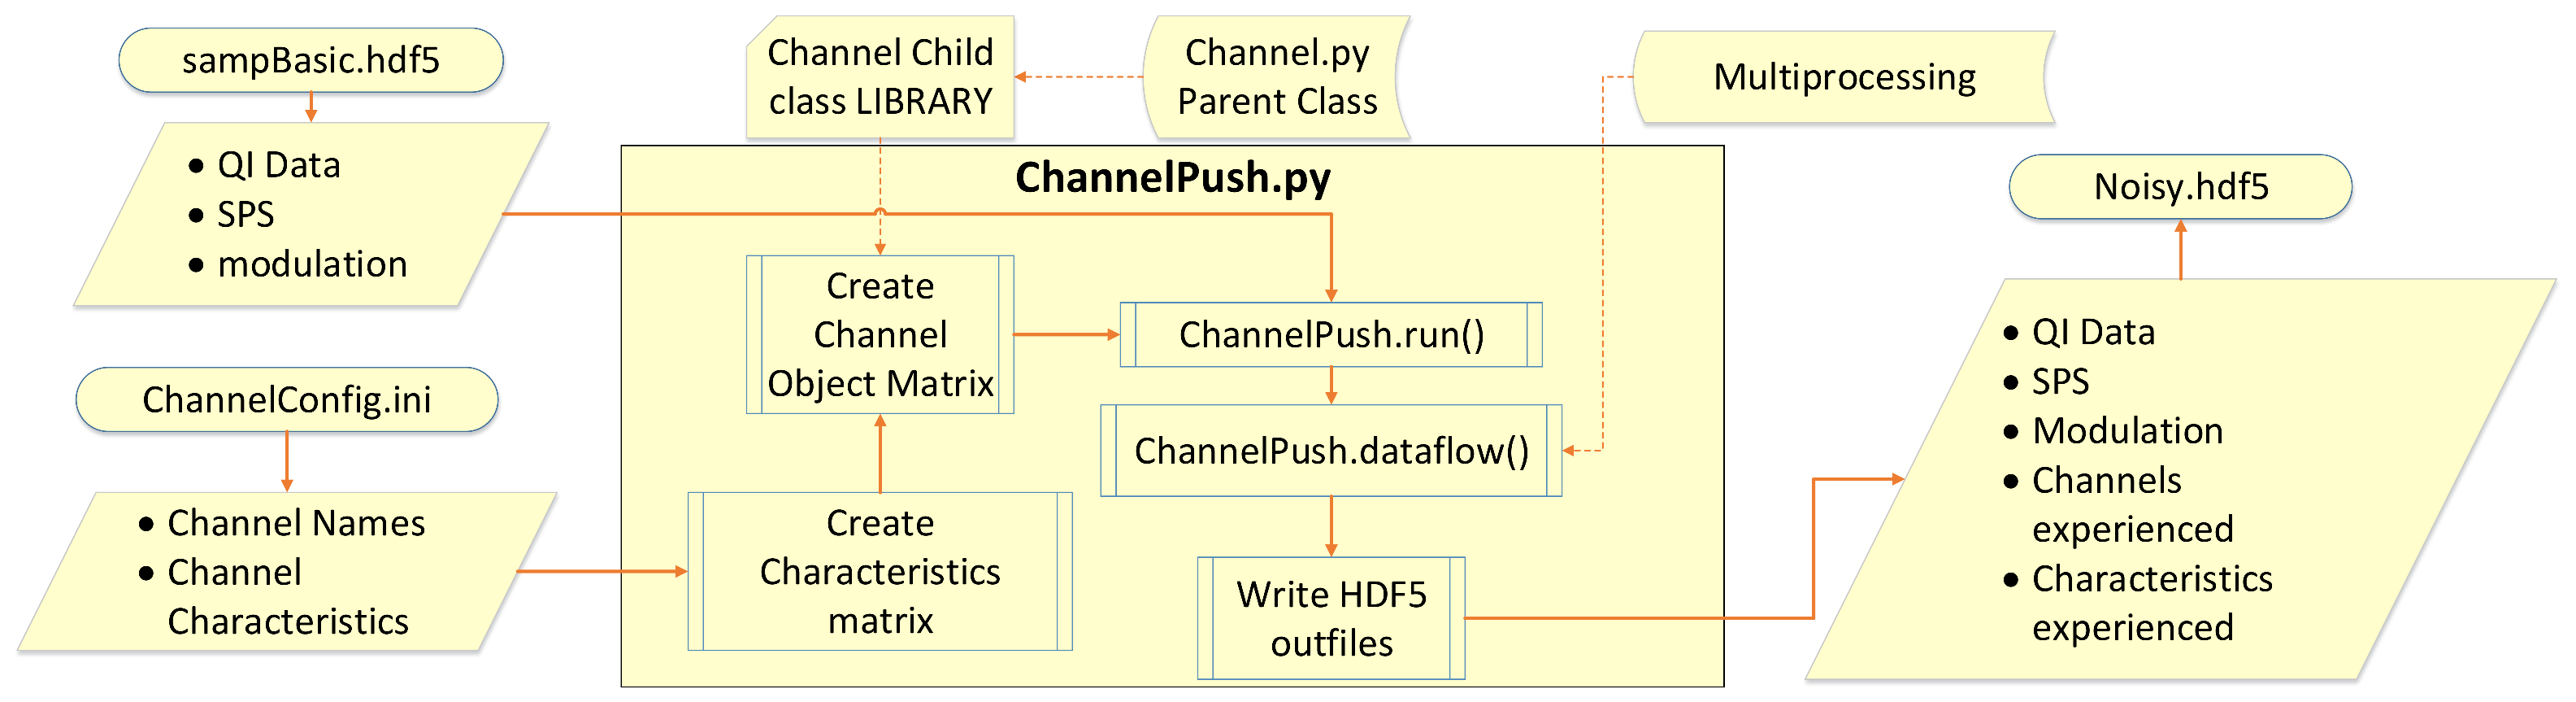
\includegraphics[width=1\textwidth,keepaspectratio]{figs/channelpush_paper.eps}
    \caption{ChannelPush.py takes in sampBasic.hdf5 and ChannelConfig.ini as inputs, and writes one or many Noisey.hdf5 outfiles. In the create channel object matrix sub-process, the channel library is used to initialize channel objects, which inherit from the channel parent class. The dataflow() function sequentially pushes data through each list of channels in parallel, making use of the Multiprocessing package.} 
\label{fig:channeltoolsub}      
\end{figure*}

Section~\ref{sec4} of this paper and \cite{8170853} display a clear need to consider the radio front end and wireless channel effects in any NN experiment. NNs must either be trained with datasets effected by channel effects or tested with datasets gathered by receivers that correct for channel effects to maintain near-peak accuracy. Either condition must be met to maintain the fundamental training assumption by expanding training datasets to represent test datasets, or to bound test datasets to represent training datasets. The latter is often preferable, as more complex training datasets always yield lower peak accuracy. Our framework generates supersets of data that can be used to help make this training decision, and to what extent training complexity should be taken for different wireless channel phenomenon. By testing NNs with supersets from our framework, certain physical layer corrections may be revealed to be unnecessary, inadequate, or overly-complex. As an example, a NN experiment makes use of a frame synchronization block created by the user to create a superset from their Dataset Under Test (DUT). A resulting conclusion on their NNs performance might be that a longer Barker Code must be used, reducing data throughput, or training must be done with a greater range of frame synchronization errors, reducing peak NN performance. This might not be an easy decision, requiring multiple uses of our framework to hypothesize, train, and evaluate NN performance and data throughput.

The inputs and outputs of the framework are described in Figure~\ref{fig:channeltoolsub}. The framework requires a DUT and instructions for which channel blocks to push the DUT through. Framework outputs are instances of the DUT that have been modified by a unique combination of channel block realizations. Any type or amount of channel blocks may be used from a library by editing the instructions. The DUT is pushed through channel blocks one sample at a time. Channel objects may be added, modified, or removed from the framework by minimal editing of the instructions. Each output is computed and written in a separate Central Processing Unit (CPU) process.

To experiment with supersets created with our framework, training and testing is done in~\cite{convnetmodrec} with Keras2, an Application programming interface (API). TensorFlow, an open-source software library that makes use of data flow graphs to perform numerical computations, is used as the backend. In our training and testing, the DUT is divided into training and testing sets, making sure there is no overlap of values. We utilize a sequential NN, which is composed of layers which only interact with their neighboring layers. Common sequential NN layers include reshape, zeropadding2D, convolutional2D, dropout, flatten, activation, and dense layers. Reshape layers adjust the height and width of layer nodes structures and batch size (which determine the number of training parameters). Zeropadding2D adds zero values to node's sides, tops, and bottoms. Convolutional2D inputs are convolved over 2 dimensions to produce a tensor of outputs functioning as hidden layers between input and output layers. Dropout layers randomly set a fraction of the inputs to 0 at each update during training to prevent overfitting. Flatten layers reduce the dimension of the input, often to reduce the last hidden layer's output shape to the smaller output layer's input shape. The activation and dense layers apply a non-linear function to inputs, most popularly a Mean Square Error (MSE) function.

Perhaps the most notable layer here is the activation layer, which applies a non-linear function to the layers inputs. During the most popular method of training, Stochastic Gradient Descent (SGD), training parameters are determined by an algorithm involving a loss function approximation. That approximation is described as a batch-normalized sum of non-linear functions. For an overview of Machine Learning (ML), the reader is directed towards section II of~\cite{8054694}

\subsection{Implementation}
\label{sec3}
In development, sampBasic.hdf5 has served as our DUT, a dataset of complex values representing constellation points of equiprobable random binary bits. In the hdf5 format, data can be assigned to subsets, and each subset, or the whole hdf5 file, assigned labels in the form of ['Key'] = value. Labels utilized are the Samples Per Symbol (SPS) or oversampling factor of the data, the source file of the dataset, the version of hdf5 the file is source encoded with, and the modulation type of the dataset. ChannelConfig.ini represents the configuration for the framework used in development. The .ini format follows a key = value format, organized under headers [HEADER], where all values are strings. Channels are described by keys 'channelx' under the [CHANNELS] header and 'characteristicsx' under the [CHARACTERISTICS] header. Each channel's characteristic parameters are '|' separated, while a sweep over that parameter's values are comma separated. Each channel realization writes a uniquely modified version of the DUT as noiseyx.hdf5. This file multiplication can extend over any number of sequential channel objects, as seen in Figure~\ref{fig:channeltoolstructure}. Each output file utilizes hdf5's labeling capabilities, detailing the types of channels and parameter values of those channels that each file was pushed through in the form ['channel:parameter'] = value.

After the configuration file is imported, delimiters convert the configuration into a 3D matrix. Within this structure, each primary index signals a channel block type, the second a parameter, and the tertiary index a value of that parameter.

\begin{figure}[ht!]
	\centering	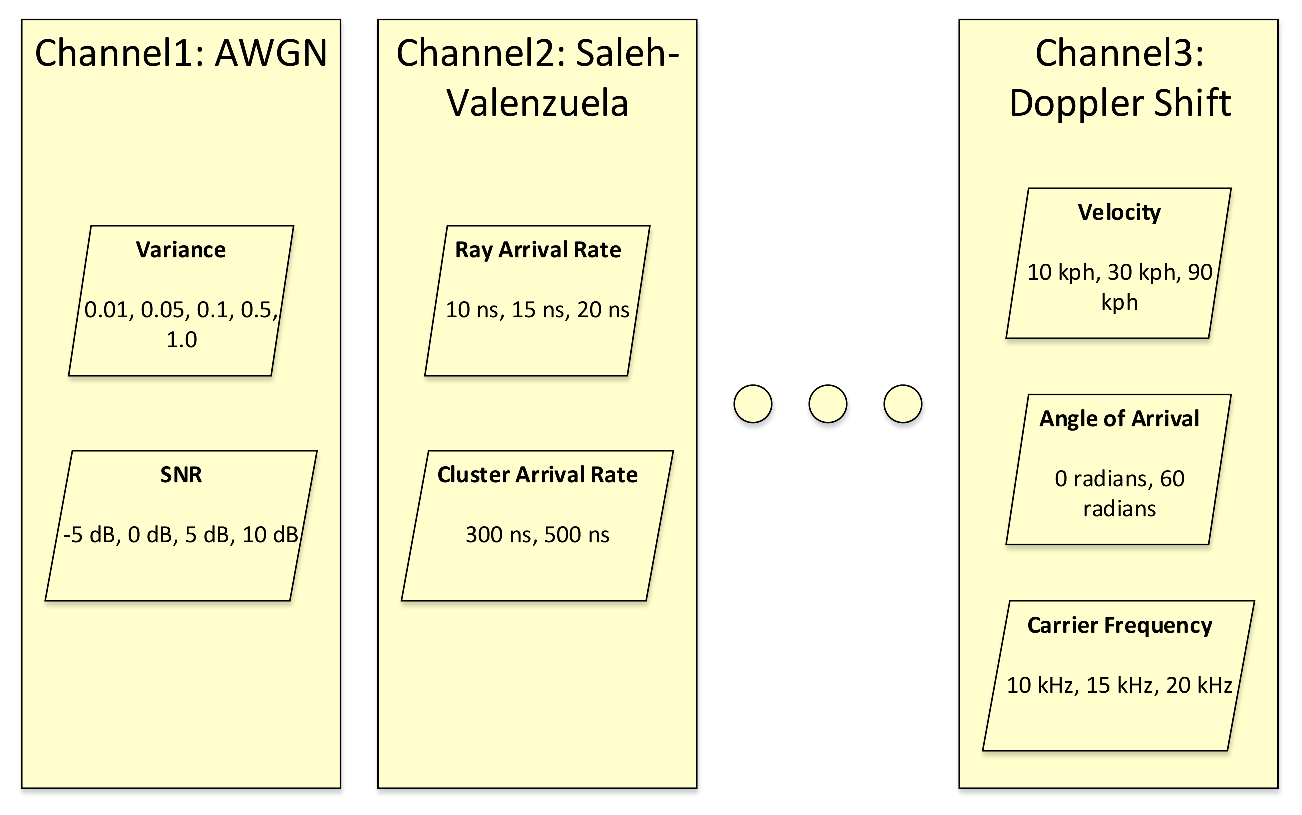
\includegraphics[width=0.45\textwidth,keepaspectratio]{figs/vtc_list_structure.eps}
    \caption{Example 2D channel matrix built from ChannelConfig.ini. There exist 20 AWGN, 6 Saleh-Valenzuela, and 18 Doppler Shift channel objects in this example, which will result in 2160 hdf5 files written. Each dataset features a unique combination of the 3 wireless channels modifying the same input dataset, with labels describing which realization was experienced} 
\label{fig:channeltoolstructure}      
\end{figure}

From that 3D matrix, a 2D matrix of channel objects is initialized, where the primary list signals grouping of channel types, and the secondary list is each realization of that channel type. Channel classes share similarities in the way they handle states, inputs, and outputs, so they inherit from a parent Channel class. A template exists to add a child channel class to the core library. in the run() function, the 2D matrix is fragmented into 1D lists of channel objects, where the total set of lists represents every possible sequential combination of unique channel realizations such that there is at least one of each channel type in each list. The next function call, dataflow(), sequentially modifies the input data by each channel of each list. This task, as well as file writing and attaching labels, is performed in parallel using the Multiprocessing import.

We modify~\cite{convnetmodrec} to run with a python3.5 interpreter instead of 2.7, using TensorFlow as a backend instead of Theano, as in the journal. The NN structure used is identical to theirs besides the dimensions of our datasets (see Table~\ref{table:tab1}). The dimension size change is due to a difference in Samples Per Symbol (SPS). The input layer has an output shape of (None, 1, 2, 4), having 4 channels as opposed to 128. This represents 4 samples of each symbol in our datasets rather than 128, where the data transmitted remains constant but probabilistic channel effects vary.

\begin{table*}[t!]
\centering
\caption{The structure of the NN used in section~\ref{sec4}. Each row represents a layer, where output shape is displayed as (batch, height, width, channels) and (batch\_size, input\_dim). Each layer is connected to the previous layer, and number of params is proportional to SPS and the size of convolutional layers.}
\begin{tabular}{c  c  c  c }
\toprule
Layer (type) & Output Shape & Param & Connected to\\\hline\hline
reshape\_1 (Reshape) & (None, 1, 2, 4) & 0 & reshape\_input\_1[0][0]\\
zeropadding2d\_1 (ZeroPadding2D) & (None, 1, 2, 8)    & 0       &    reshape\_1[0][0]\\
conv1 (Convolution2D)          &  (None, 256, 2, 6)  & 1024     &   zeropadding2d\_1[0][0]\\            
dropout\_1 (Dropout)            &  (None, 256, 2, 6)  & 0         &  conv1[0][0]\\
zeropadding2d\_2 (ZeroPadding2D) & (None, 256, 2, 10)  & 0          & dropout\_1[0][0]\\                 
conv2 (Convolution2D)          &  (None, 80, 1, 8)   & 122960     & zeropadding2d\_2[0][0]\\          
dropout\_2 (Dropout)           &   (None, 80, 1, 8)  &  0          & conv2[0][0]\\                  
flatten\_1 (Flatten)           &   (None, 640)      &   0          & dropout\_2[0][0]\\                 
dense1 (Dense)               &    (None, 256)       &    164096    & flatten\_1[0][0]\\                
dropout\_3 (Dropout)          &    (None, 256)      &     0          & dense1[0][0]\\                  
dense2 (Dense)               &    (None, 11)      &      2827       & dropout\_3[0][0]\\              
activation\_1 (Activation)   &     (None, 11)     &       0          & dense2[0][0]\\                 
reshape\_2 (Reshape)        &      (None, 11)    &        0    &       activation\_1[0][0]\\\hline\hline
Total params\: 290,907\\
Trainable params\: 290,907\\
Non-trainable params\: 0\\
\hline
\bottomrule
\end{tabular}
\label{table:tab1}
\end{table*}

\subsection{Simulation and Results}
\label{sec4}

In this paper, we focus on the wireless channel effect of CFO and phase ambiguity due to their computational simplicity. In any communication system, the transmitter and receiver typically are not using the same Local Oscillator (LO). This leads to issues in the baseband when a received signal is demodulated from its carrier frequency, proportional to the max possible frequency offset:

\begin{equation}
\label{eq3}
f_o,_{max} = \frac{f_c \times PPM}{10^6}
\end{equation}

\noindent where PPM is the maximum possible Parts Per Million offset of the LO, and $f_c$ is the received signal carrier frequency. We investigate the performance of~\cite{o2016convolutional} when the 2016.10a dataset has the additional channel effect of CFO, uncorrected by classical Coarse Frequency Correction (CFC) and Fine Frequency Correction (FFC) methods. As shown in~\cite{8170853}, testing done against channel effects not trained with causes classification accuracy to significantly decrease. We have observed a relationship between the complexity of the environment a NN is trained for and peak accuracy. Consequently, it should be the goal of any additional complexity in NN physical layer datasets to represent expected channel effects realistically. To obtain a realistic PDF of CFOs for training, ideally an infinite number of random values would maximize accuracy. However, training is very computationally expensive, so such a goal is unrealizable, particularly when the proposed framework is considered (as each additional channel type can represent one, or several, orders magnitude additional samples). Considering this, the datasets in Table~\ref{table:tab2} are presented to learn more about practical performance of the classifier~\cite{o2016convolutional}.

\begin{table}[ht!]
\centering
\caption{Four datasets generated with our framework. Datasets are trained, partitioned, and tested against a modulation classifier.}
\begin{tabular*}{0.5\textwidth}{c l c }
\toprule
Dataset & Description\\\hline
RML\_4sps & RML2016.10a dataset at 4 SPS and 0 CFO\\
CFO\_grc & RML\_4sps trained with GRC's dynamic channel\\
CFO\_super & RML\_4sps file multiplied over 100 discrete CFOs channels\\
 & evenly spaced from 0 to 20\% normalized to sample rate\\
Phase\_super & RML\_4sps file multiplied over 100 phase ambiguities evenly\\
 & spaced from 0 to $2\pi$ radians\\
\bottomrule
\end{tabular*}
\label{table:tab2}
\end{table}

The RML2016.10a dataset contains 1000 symbols, oversampled by a factor of 128, passed through GRC's dynamic channel model object, which has an 8-tap multipath profile of K-factor 4, fixed Doppler shift 1 Hz, random STO of variance 0.01 max value 50 samples, and random CFO of variance 0.01 max value $0.25\%$ normalized to 200 kHz sample rate. The dataset contains 11 modulation schemes (8 digital, 3 analog). SNR is swept from -20 dB to 20 dB in 2 dB steps. The CFO alter each sample of each dataset with the following phase rotation per sample:

\begin{equation}
\label{eq1}
\Theta[i] = e^{j\frac{0.2\times i}{N}\frac{2\pi}{sps}}
\end{equation}

\noindent where $N$ is the number of CFO values, $i = 0, 1...N-1$, and $sps$ is the oversampling factor. Since frequency is known as phase over time, the phase rotation at sample $k$ in a dataset for constant SNR, modulation type, and phase rotation per sample can be written as:

\begin{equation}
\label{eq4}
\phi[k, i] = \Theta[i]^k,~k=1,2...M
\end{equation}

\noindent where $M$ is the number of samples in a transmission with the above mentioned constants, and $\phi$ is only a function of $i$ for the phenomenon of initial phase offset. The CFO\_super test set aims to provide complete coverage of all possible CFO outcomes, making testing more reproducible and consistent. In Figure~\ref{fig:nocfo}, we present the accuracy of~\cite{o2016convolutional} in classifying the modulation scheme of data trained by RML\_4sps and tested by CFO\_super, data trained by CFO\_grc in Figure~\ref{fig:cfo}, and data trained by RML\_4sps and tested by Phase\_super in Figure~\ref{fig:phase}.

\begin{figure}[ht!]
	\centering	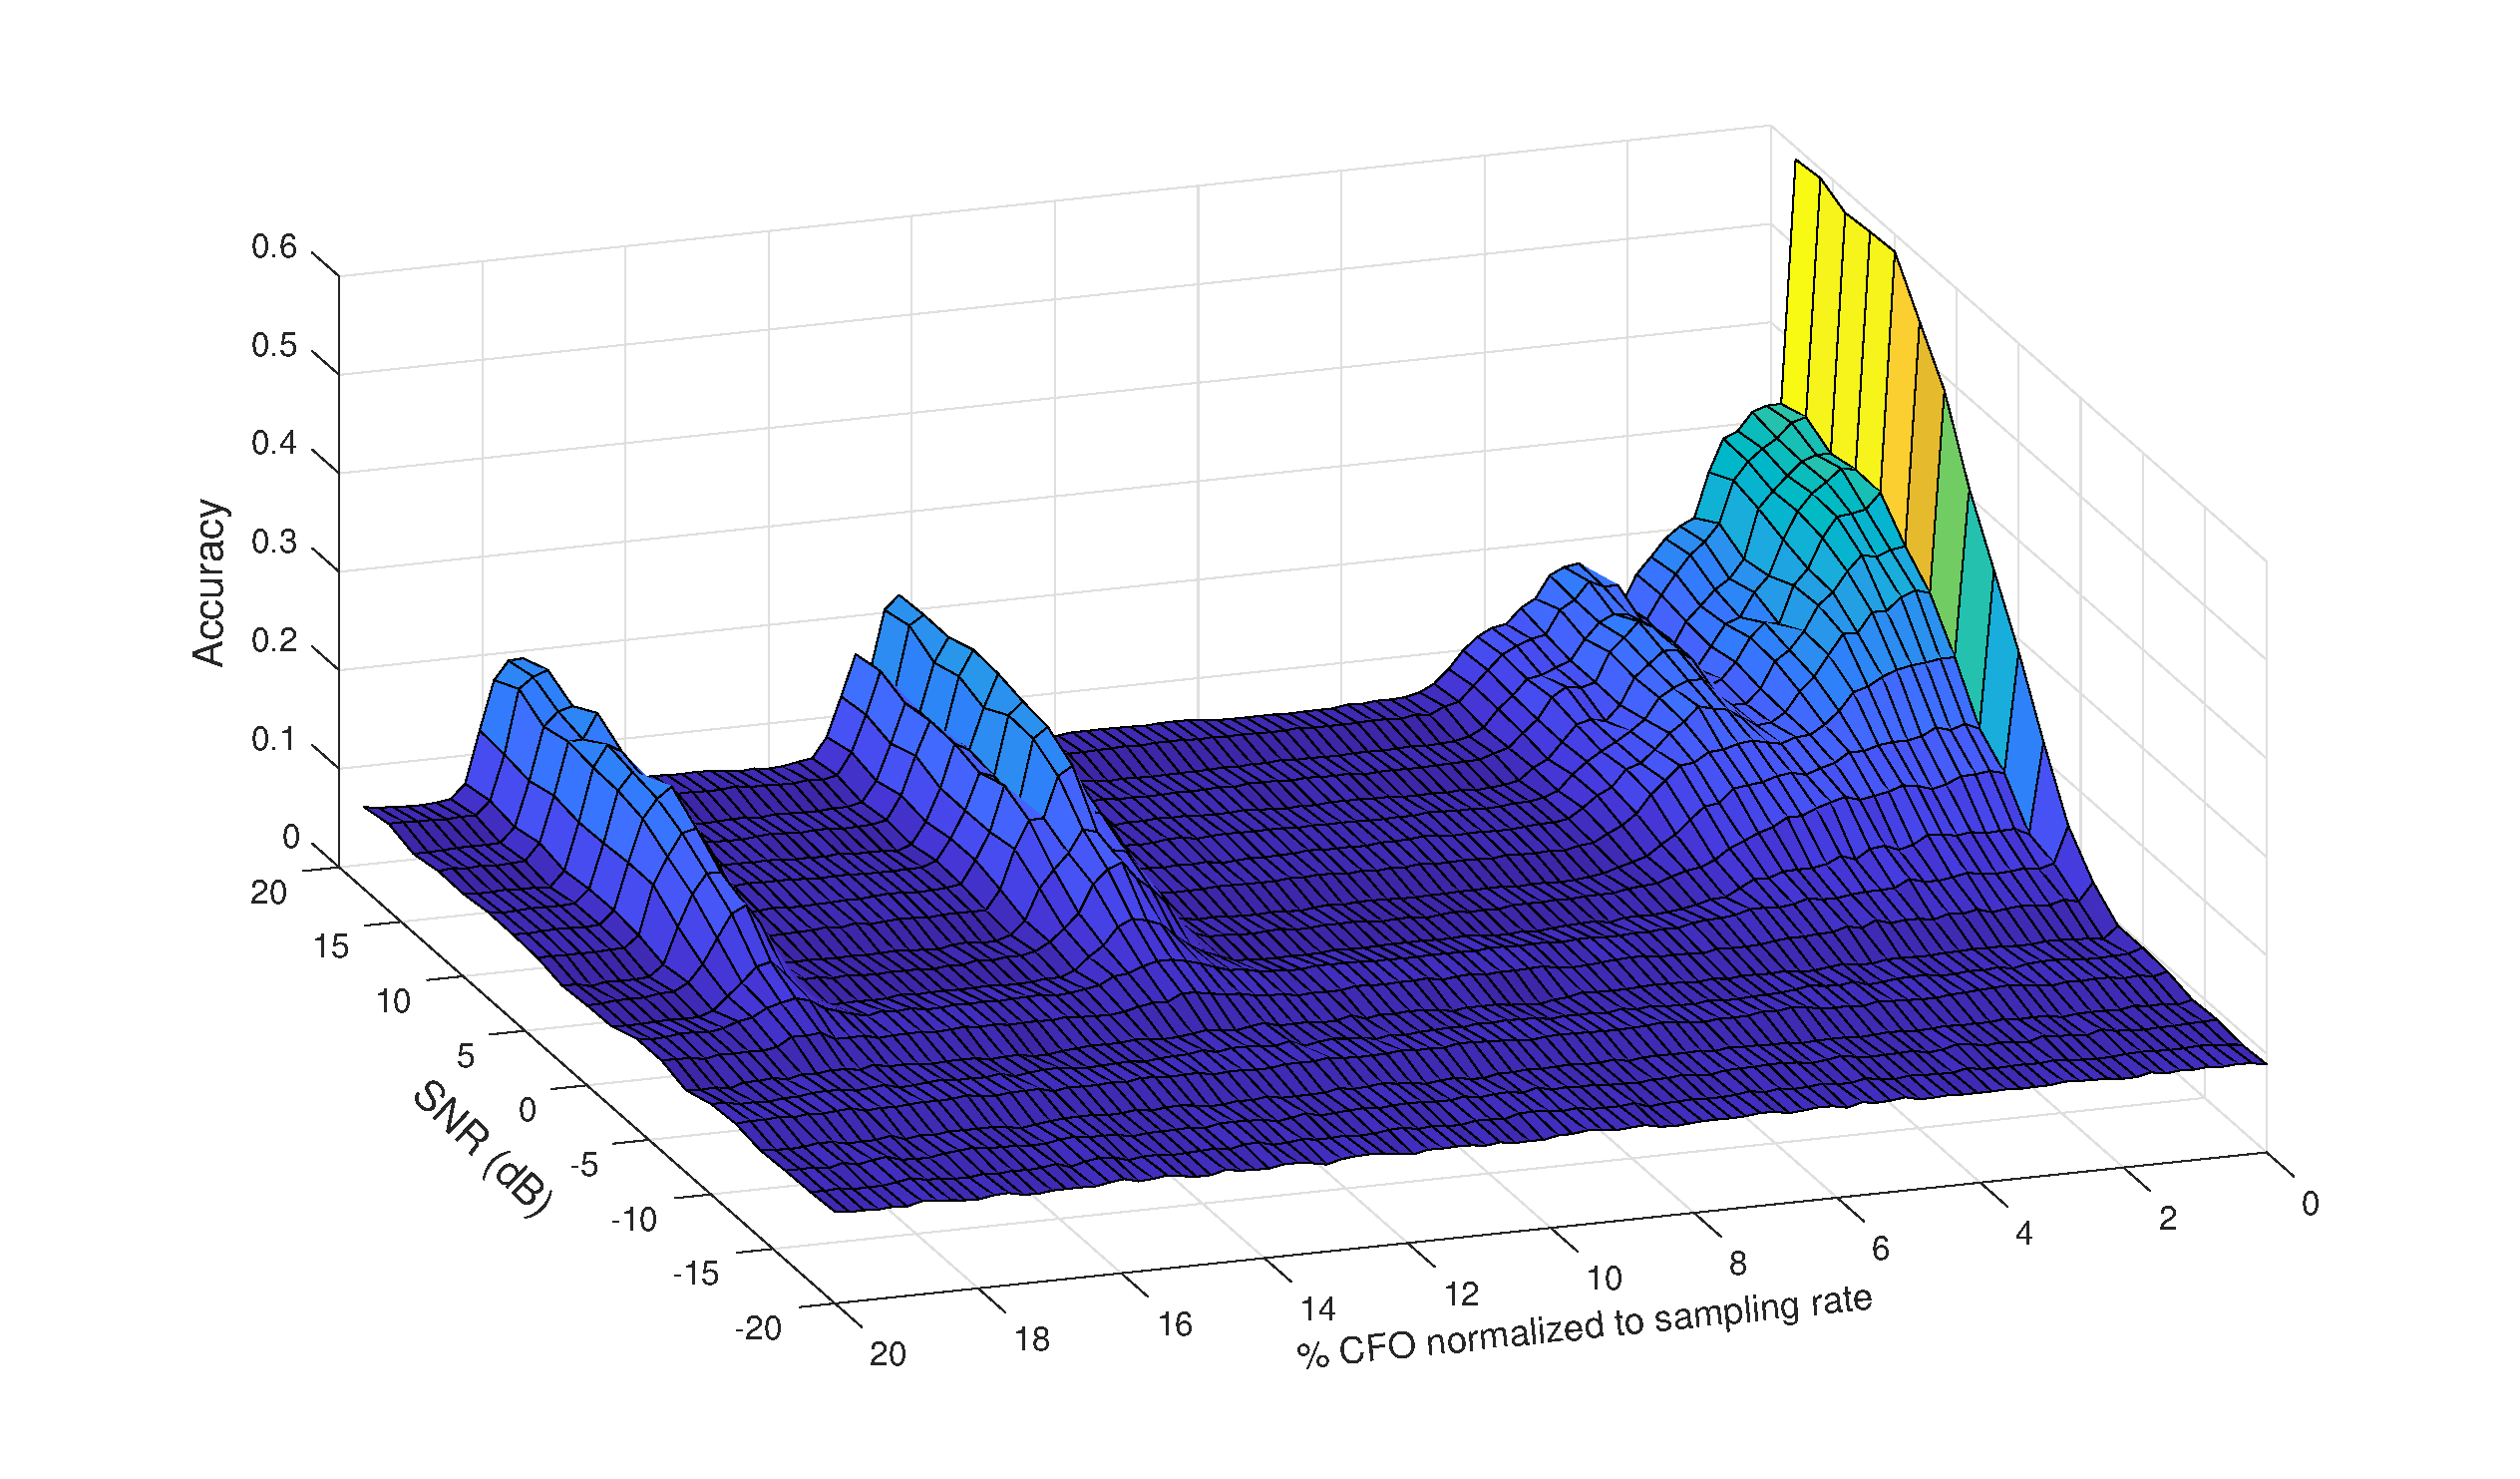
\includegraphics[width=0.45\textwidth,keepaspectratio]{figs/rml2016_nocfo.eps}
    \caption{CFO\_super test results when trained with RML\_4sps. Accuracy is averaged over 11 modulation schemes, and significantly decreases when tested against a CFO channel of just $0.2\%$ normalized to sample rate. Accuracy peaks at $60\%$.} 
\label{fig:nocfo}      
\end{figure}

\begin{figure}[ht!]
	\centering	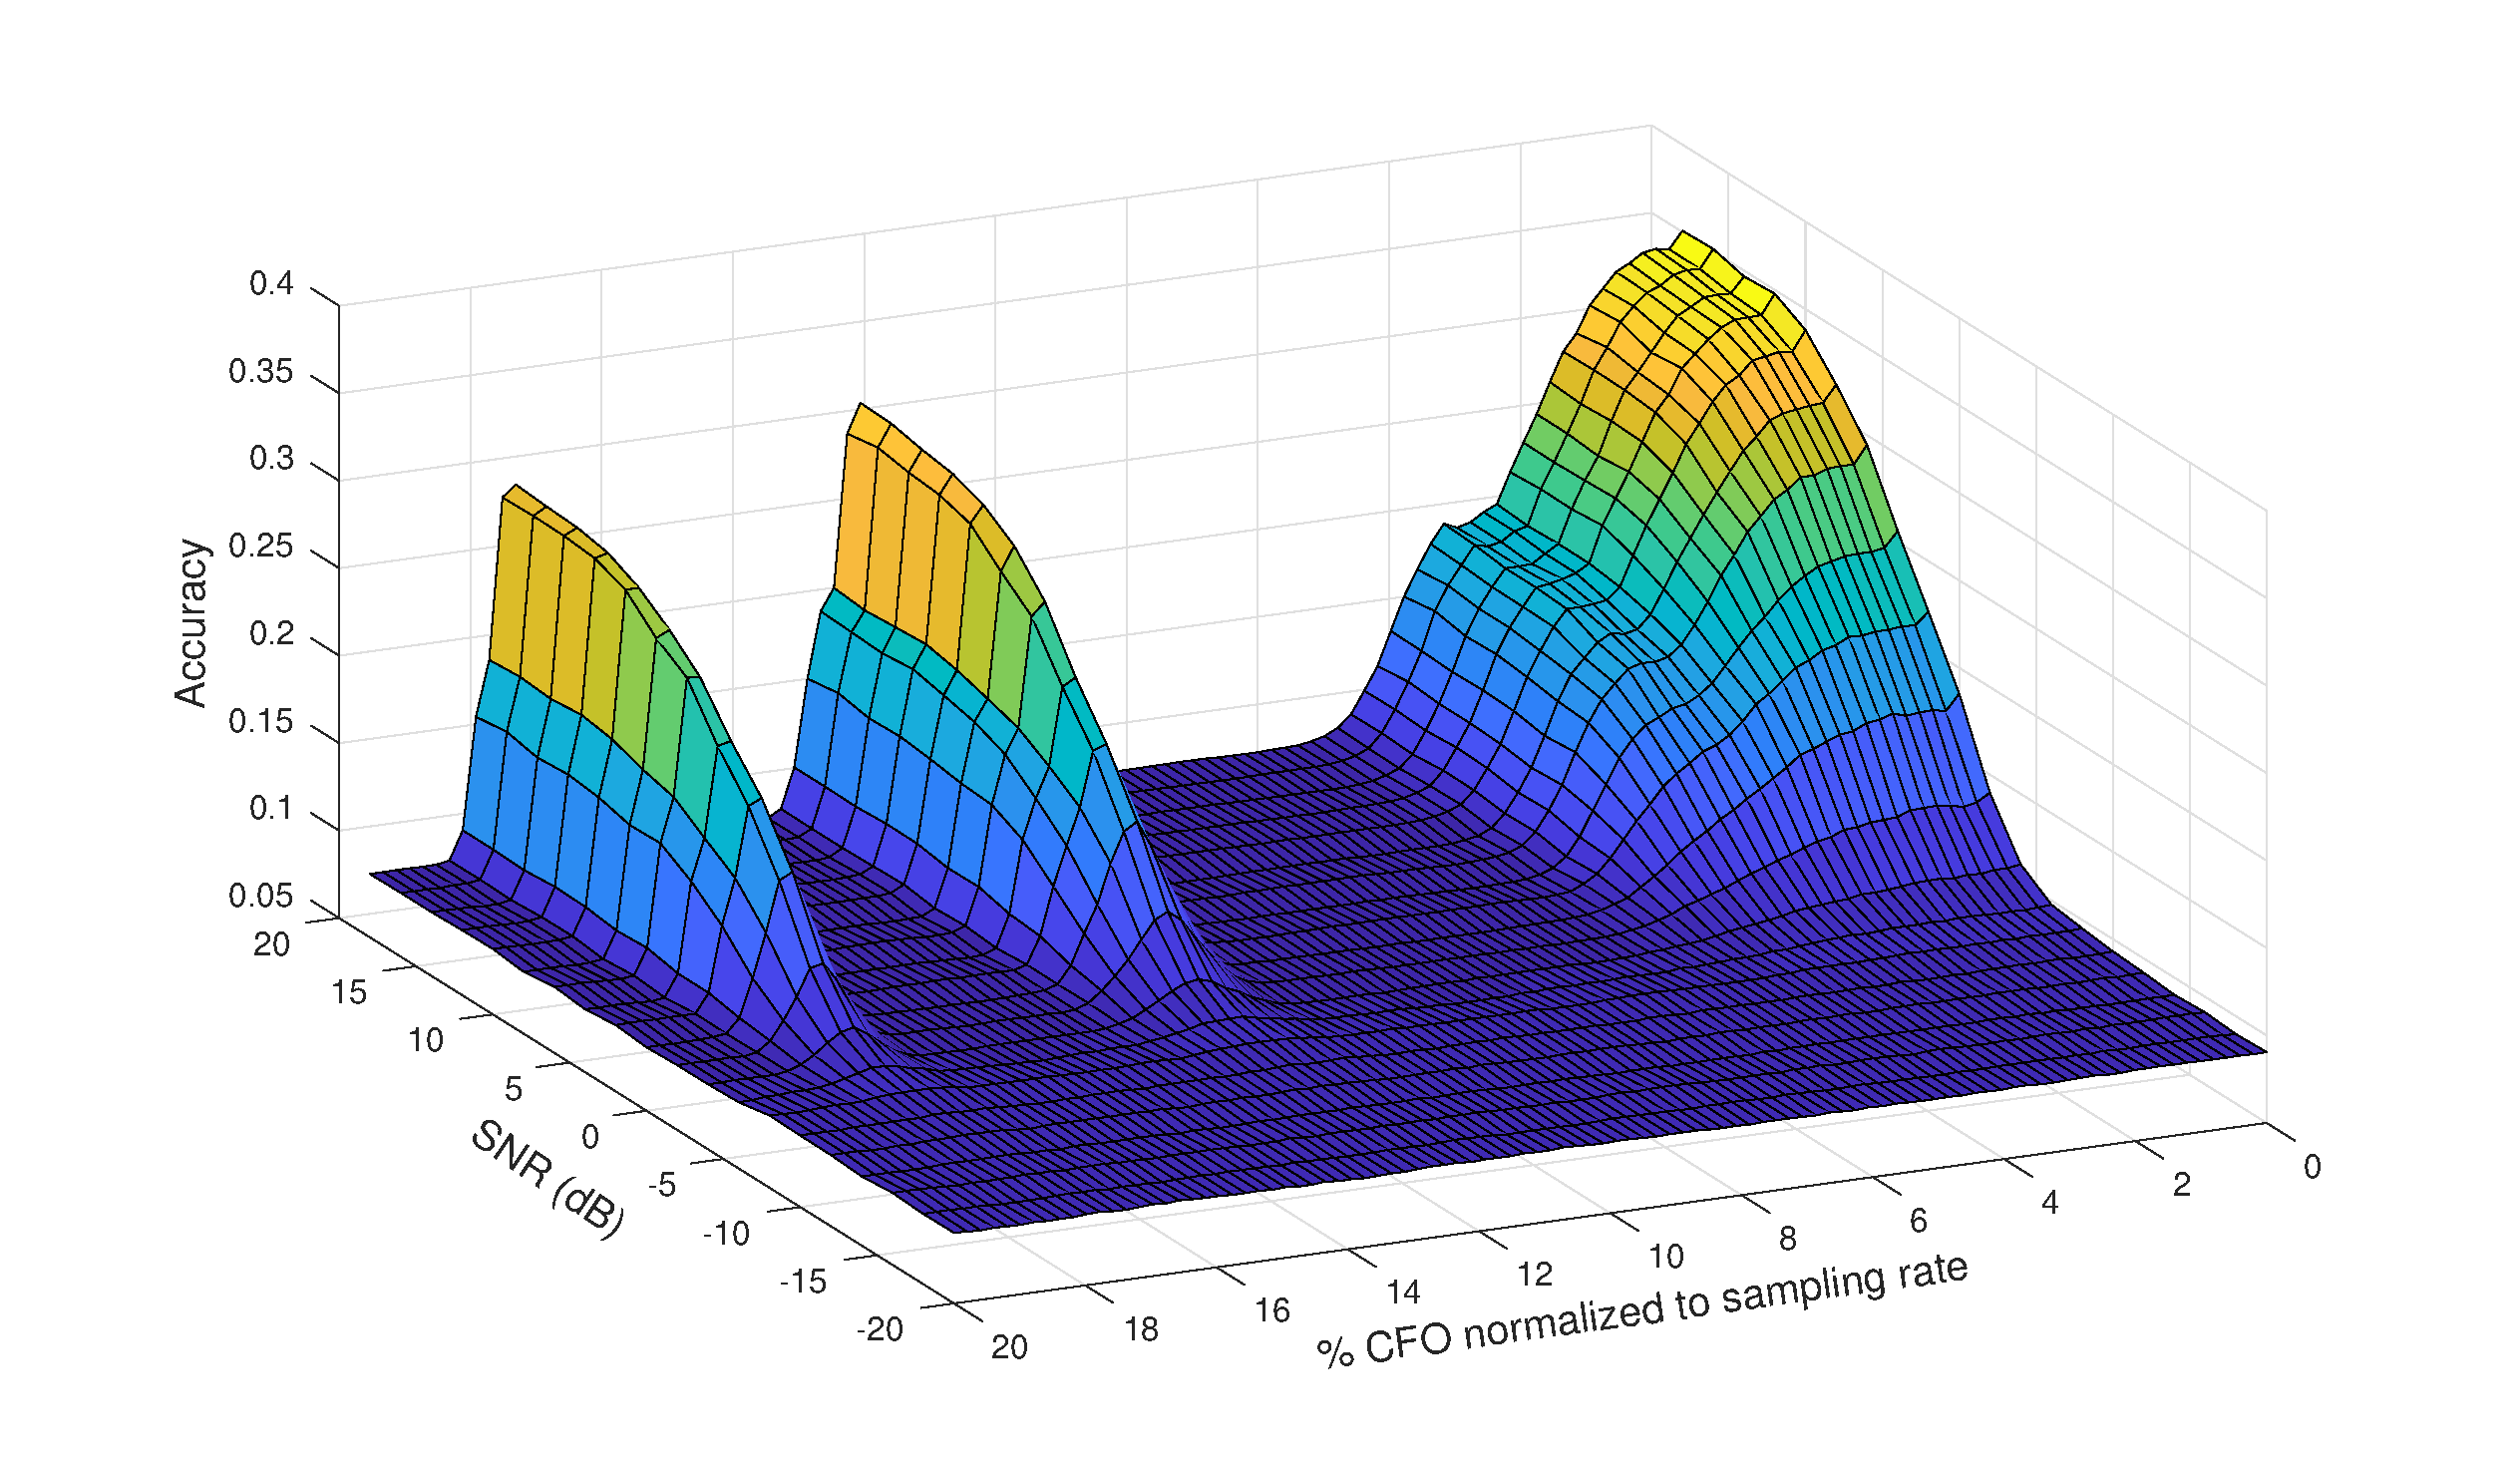
\includegraphics[width=0.45\textwidth,keepaspectratio]{figs/rml2016_tencfo.eps}
    \caption{CFO\_super test results when trained with CFO\_grc, as in the original 2016 dataset. Accuracy is averaged over 11 modulation schemes, and significantly decreases when tested against CFO channels of more than $1\%$ normalized to sample rate. Accuracy peaks at $38\%$.} 
\label{fig:cfo}      
\end{figure}

\begin{figure}[ht!]
	\centering	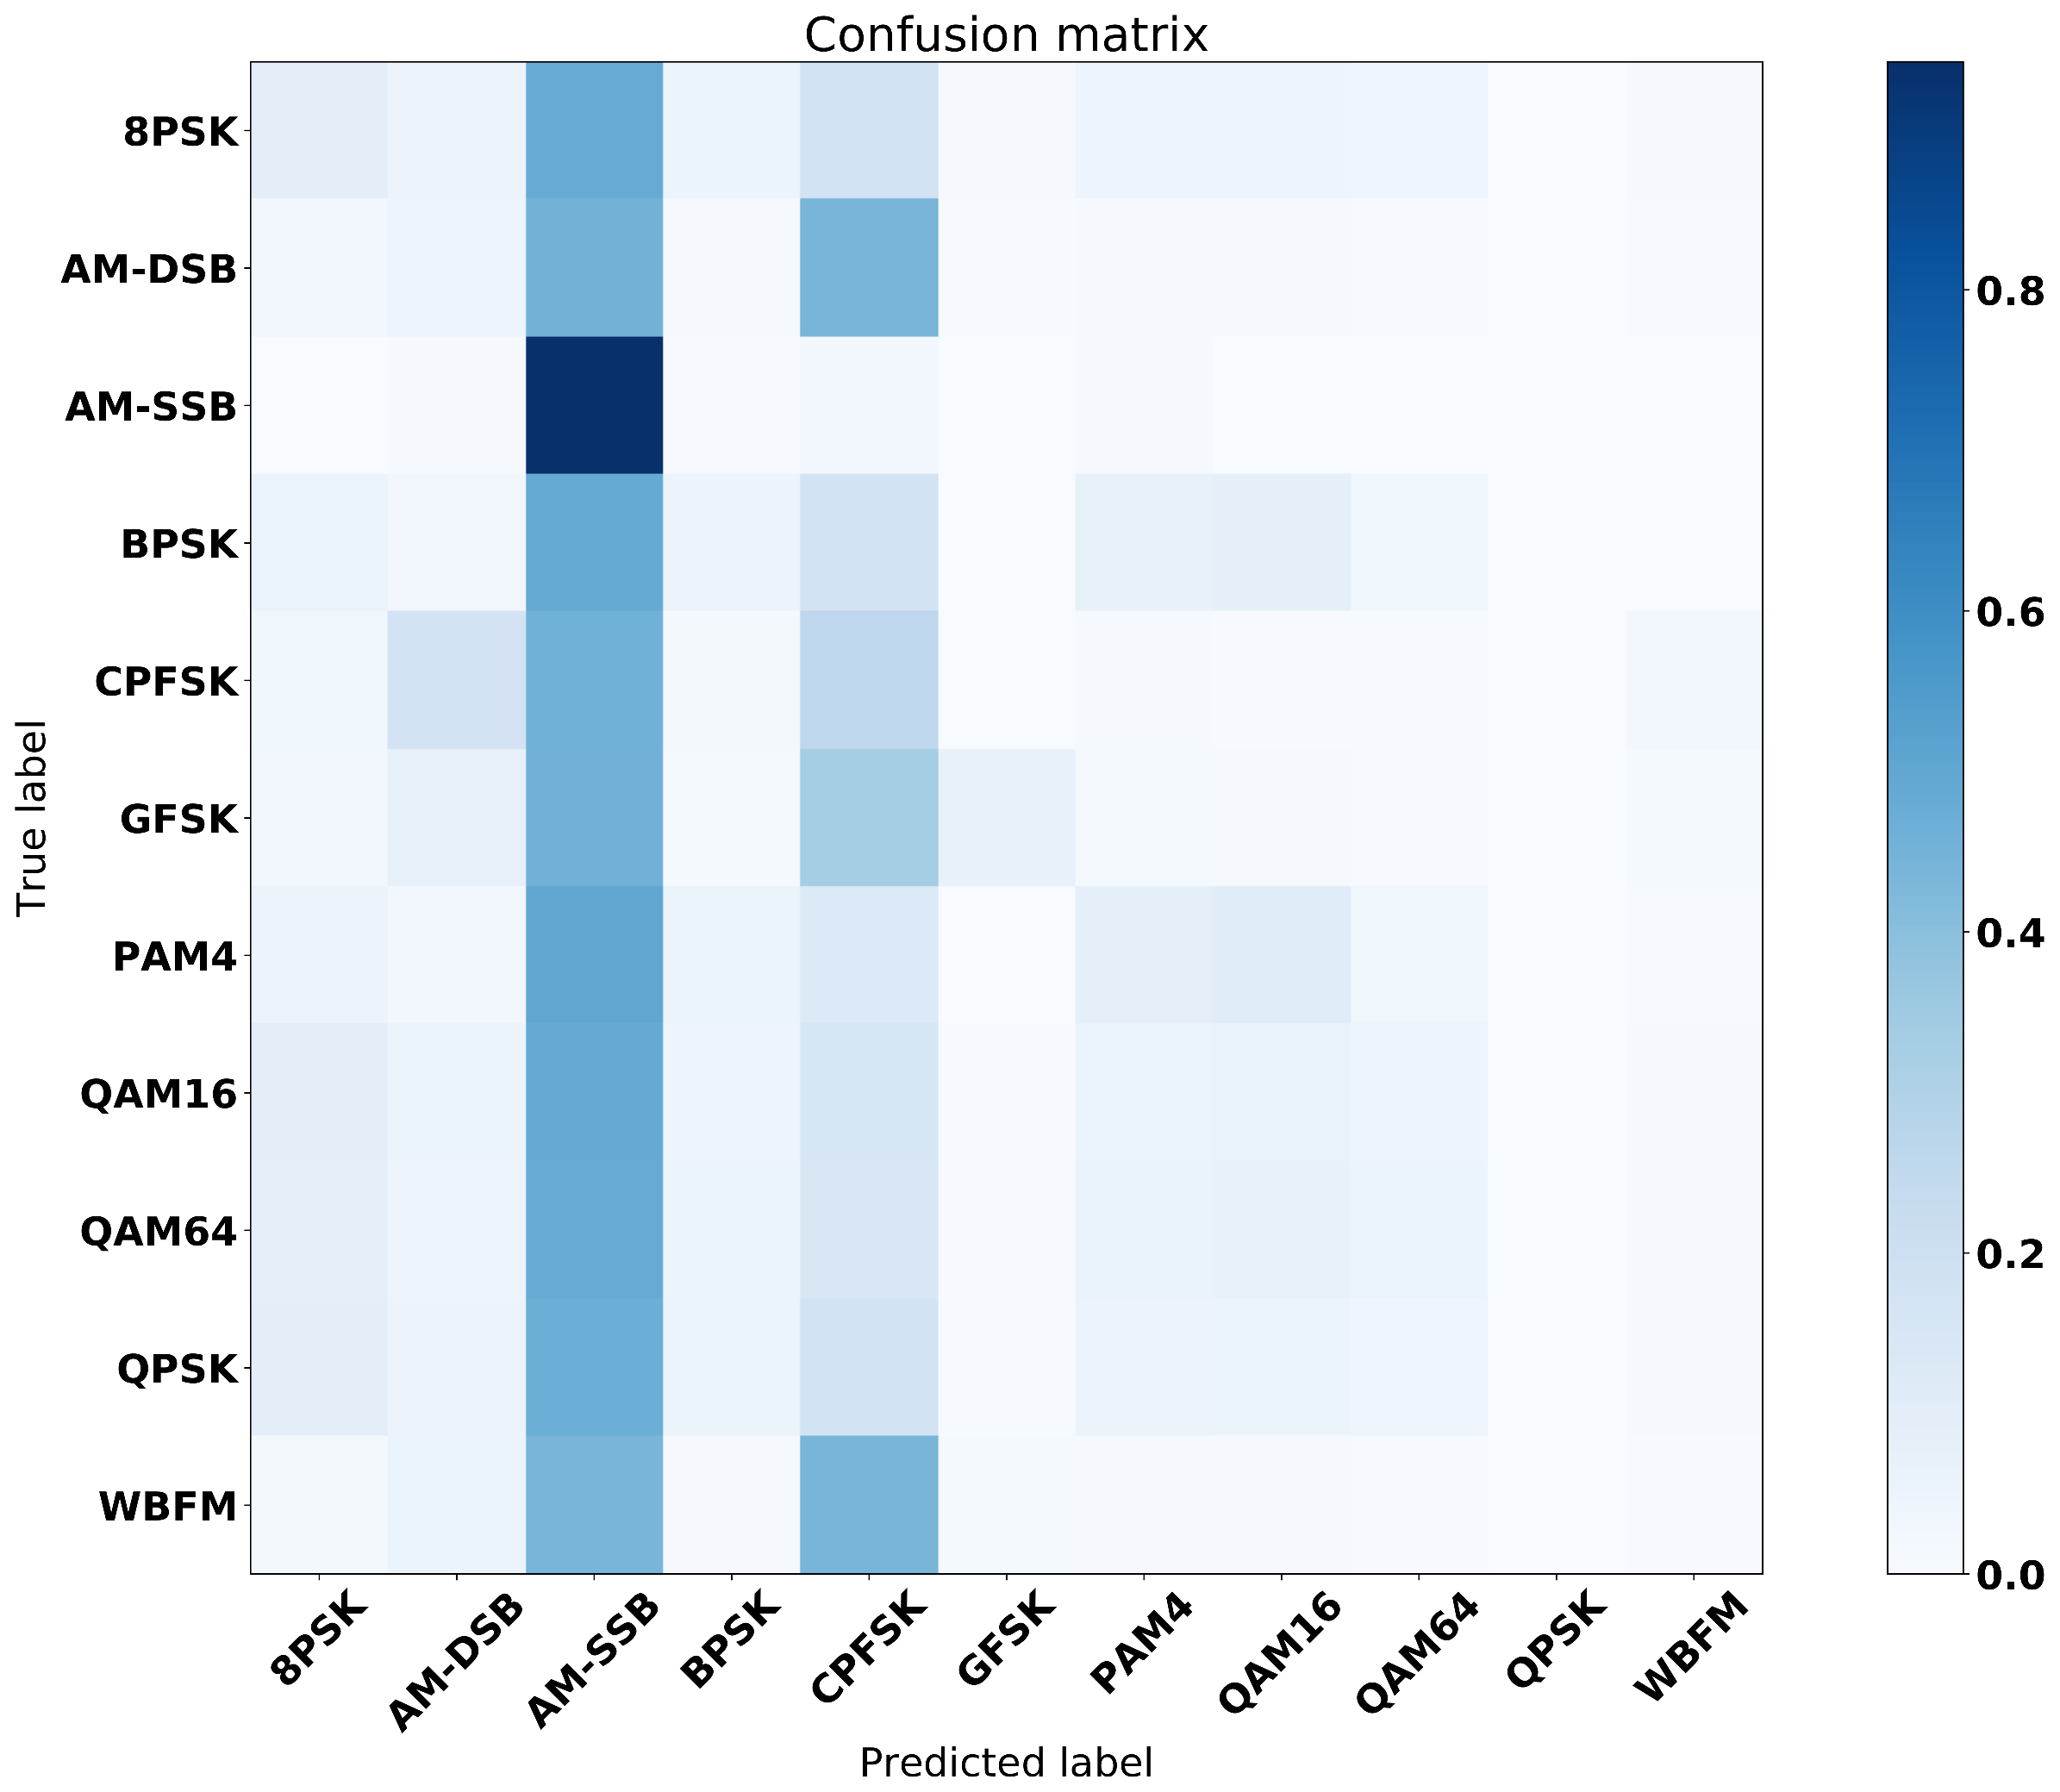
\includegraphics[width=0.45\textwidth,keepaspectratio]{figs/confusion.eps}
    \caption{CFO\_super confidence matrix for $12.53\%$ CFO averaged over SNR, see Figure~\ref{fig:cfo}. AM-SSB is the predicted label at low SNR values as when there is no CFO, and often correctly predicts CPFSK at higher SNR values. This seems to imply certain periodic CFO values do not affect the appearance of CPFSK constellation plots.} 
\label{fig:confusion}      
\end{figure}

Since the classifier is shown in confusion matrices to guess AM-SSB when SNR is low, resulting classifier accuracy nears $9.09\%$. The accuracy values peak when there is no CFO and sharply decreases as CFO grows in Figure~\ref{fig:nocfo}. The small improvement in accuracy at high SNR values and CFO values of $12.53\%$ and $17.78\%$ in Figure~\ref{fig:cfo} are due to the classifier correctly predicting the modulation scheme is Continuous Phase Frequency Shift Keying (CPFSK). Although accuracy improvement is small, if the classifier is only used to decide between CPFSK and a few other modulation schemes rather than 11, the accuracy increase would be much more significant, perhaps enough for the CFO correction to be relaxed or removed. Figure~\ref{fig:nocfo} reveals that the classifier does not perform with more than $0.2\%$ CFO when trained with RML\_4sps, which is problematic. Figure~\ref{fig:cfo} displays, as shown in~\cite{8170853}, the peak accuracy dropping due to the added complexity of the data from about $60\%$ to $40\%$, but that accuracy now stretches to $1\%$ CFO normalized to sample rate. A training decision here is to identify the CFO  (\ref{eq3}) of the system used in experimentation, and train the classifier for CFOs no greater than that to maintain peak accuracy.

Given the uniform distribution of initial phase offset in radio communications, Figure~\ref{fig:phase} reveals significant drops in accuracy at many phase offset values. Consequently, this classifier would likely require phase correction through either codewords, differential encoding, or equalization to see consistent near-peak performance.

\begin{figure}[ht!]
	\centering	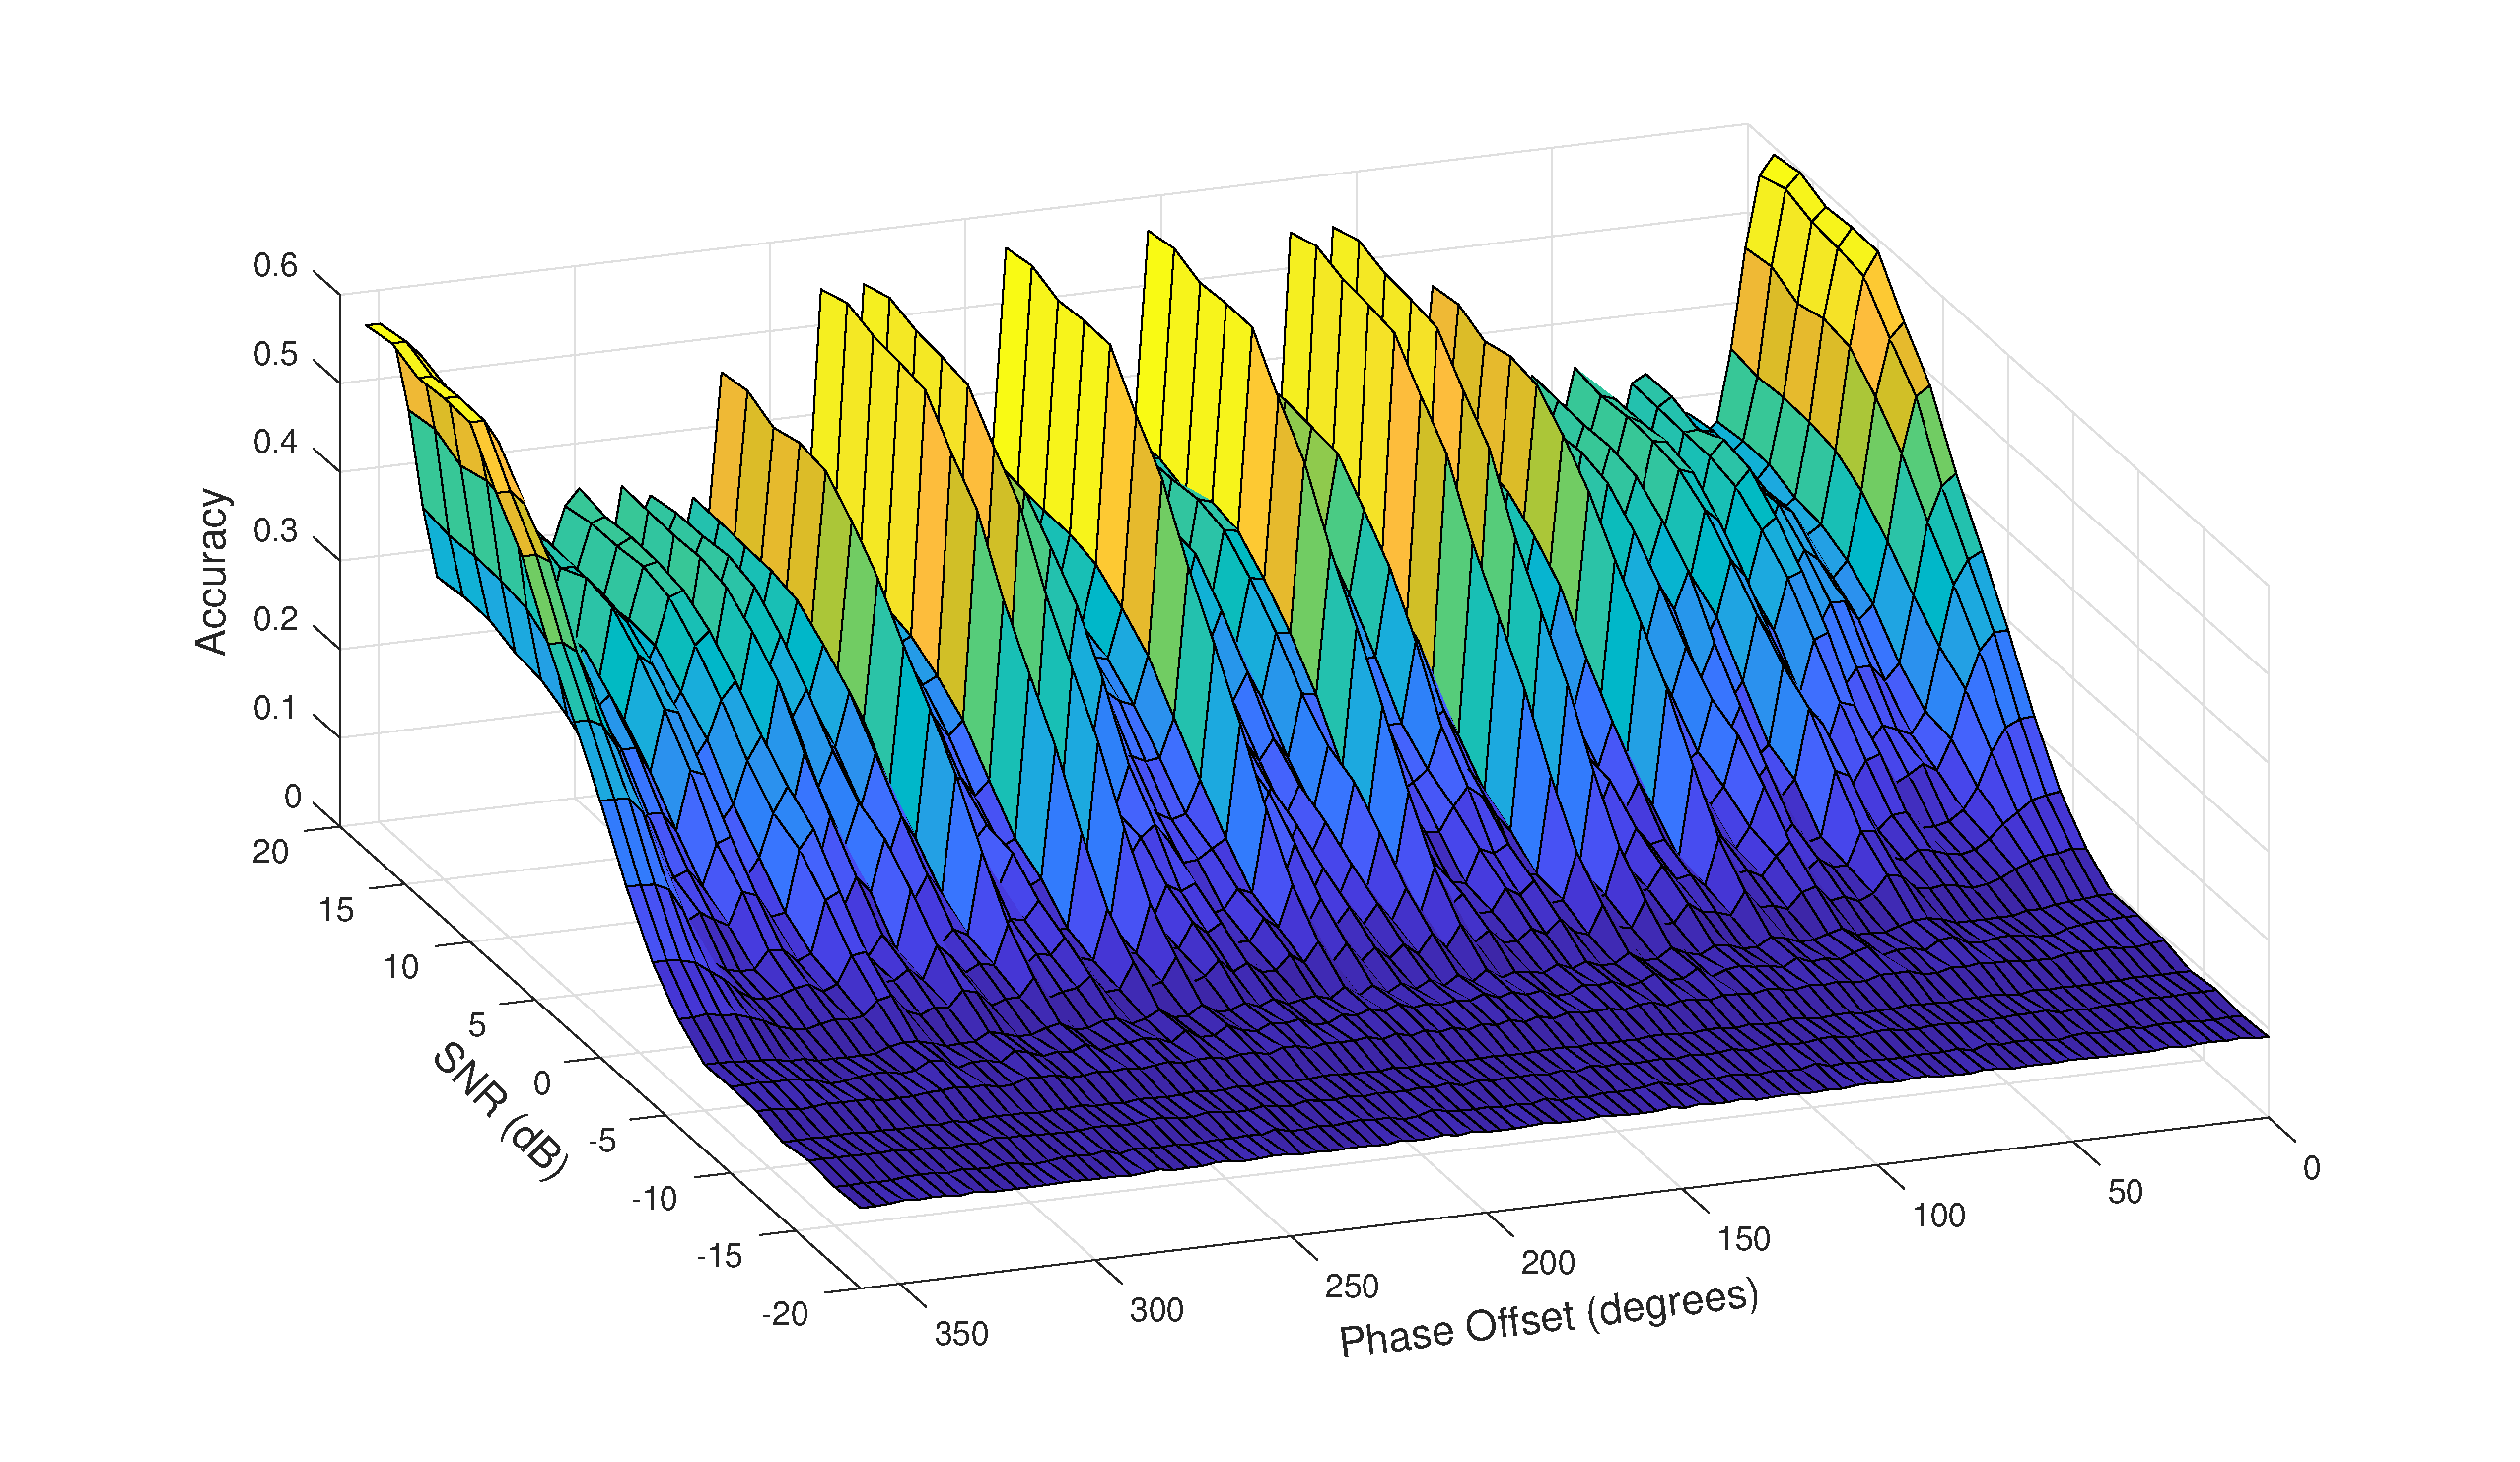
\includegraphics[width=0.45\textwidth,keepaspectratio]{figs/phase_sweep.eps}
    \caption{Phase\_super test results when trained with RML\_4sps. Accuracy is averaged over 11 modulation schemes, and remains close to peak performance for phase offsets of less than 4 degrees and certain discretized values. $60\%$ peak accuracy can drop by as much as half for many phase offset values.} 
\label{fig:phase}      
\end{figure}

\subsection{Summary}
\label{sec5}
In section~\ref{sec1}, we described the usefulness of NNs in the communications community, and referenced an overview of recent publications. In section~\ref{sec2} the frameworks's structure was discussed, and the implementation details of RadioML and our framework were visited in section~\ref{sec3}. Finally, section~\ref{sec4} displayed simulation results using NN datasets modified by our framework.

Our proposed framework showcases an ability to identify NN testing and training decisions, and hypothesize and test for answers to what extent training complexity should be taken for different wireless channel phenomenon. Future work aims to generate multi-user supersets from lists of DUTs, where channel blocks applied to different transmissions are related by correlation factors.
